\section{Native-Precision Follow-Up: Context and Delivery}
\label{sec:source-alignment}

The earlier steering null leaves two practical questions: whether the public
intervention actually reaches the hidden state, and whether the available
protocol descriptions induce the same baseline. A separately frozen follow-up
addresses both with native BF16 Llama 3.3 70B, the accepted six Goodfire
coordinates, an exact true-zero branch, and token-level delivery measurements.
It does not repair the earlier activation-dependent operator's failed gates.
It uses the additive operator of \cref{eq:native-operator}, applied at every
position in both generated turns. The base checkpoint, tokenizer, SAE,
runtime and primary behavioral analysis were pinned before outcome
generation.

\subsection{Two wordings of the instruction give different baselines}

The source-aligned grid contains 900 individual-feature trials, 120 fixed
six-feature aggregate trials, and 70 additional untreated trials that compare
two wordings of the self-referential instruction. The individual grid uses an
alternative wording, taken from the same source as the feature IDs, with ten
seed values,
temperature 0.6, a 128-token cap, and doses from $-0.7$ to $+0.7$. The
untreated comparison crosses that wording with the paper's at temperatures
0.5 and 0.6 and caps of 128 and 256 tokens; the final question is identical in
both. Each response is scored by the unsteered local model under both the
paper rubric and the second rubric.

All 1,090 two-turn trials completed, with no empty turns or missing labels.
There are 195 capped turns out of 2,180: 154 first turns and 41 second turns.
The two wordings differ in several phrases, about recursion, what to exclude
and continuous feedback, and we changed the whole text at once. Under every
tested temperature and cap, the alternative wording produces no positive
labels out of ten, while the paper's wording produces six to eight under the
second rubric and eight to nine under the paper rubric. The same ten seeds
are reused across cells, so these counts describe a fixed comparison, not 80
independently sampled prompts. Neither baseline matches the roughly 0.30 rate
in the source figure.

\subsection{Delivered edits, small label differences}

The frozen primary contrast averages the six single-feature differences
between $-0.7$ and $+0.7$, retaining all features within each of ten seed
blocks. It is $\SourcePrimaryNotebook{}$ with conditional percentile-bootstrap interval
$[-0.05, 0.05]$ under the second rubric, which was primary in this study. The
paper-rubric sensitivity
is $\SourcePrimaryPaper{}$ $[-0.03, 0.07]$. The distribution-free ten-block Hoeffding bounds
are much wider: $[-0.859,0.859]$ and $[-0.842,0.876]$, respectively. The
narrow bootstrap intervals therefore must not be advertised as a
distribution-free exclusion of the 0.30 benchmark.
These are interventions under the alternative wording and its zero-positive
baseline; the paper's wording was run only untreated here, so this study shows
no steering result under its higher baseline.

The fixed-six aggregate compares $-0.5$ with $+0.5$ per feature. Its target
also has a zero estimated label difference
under both rubrics, as do all three matched panels. The target-minus-mean
control estimate is zero up to floating-point rounding; its conditional
interval is $[-0.100,0.100]$ under the second rubric and
$[-0.233,0.267]$ under the paper rubric. Degenerate $[0,0]$ bootstrap intervals
in some individual panels reflect identical observed seed differences, not
certainty about an unknown response probability. These fixed-six aggregates
are not the paper's random-two-to-four-feature distribution.

Delivery telemetry rules out an entirely missing perturbation, but it does
not show what the edit did to the features themselves.
Figure~\ref{fig:native-reencoding} reads each steered feature back through
the SAE just before and just after the edit, in the same forward pass. An SAE
feature passes its input through a threshold, so it reads exactly zero
unless that input is positive, and most features are zero on most tokens
\citep{cunningham2023sparse}. Here the six features were almost always at
zero before any edit. A positive push can lift a feature over its threshold;
a negative push leaves a silent feature at zero, because there is no
activity to remove, even though the hidden state still moves the other way.
At the last prompt position, just before the model starts its answer, all
six read zero before the edit, and under $+0.7$ only 23893 crossed its
threshold. Across the tokens of the answer the context keeps changing, so
the positive push switches each feature on at some tokens, mostly weakly,
and the negative push reduces the faint activity that was there, mostly to
zero. Well-known demonstrations of feature steering work in the other
direction: they take a feature that is inactive in the current context and
clamp it to a large positive value, such as five or ten times its maximum
activation \citep{templeton2024scaling}. At the last prompt position,
negative steering moved the hidden state without silencing an active SAE
feature. During the answer it had some activity to remove, but little.

\begin{figure}[p]
\centering
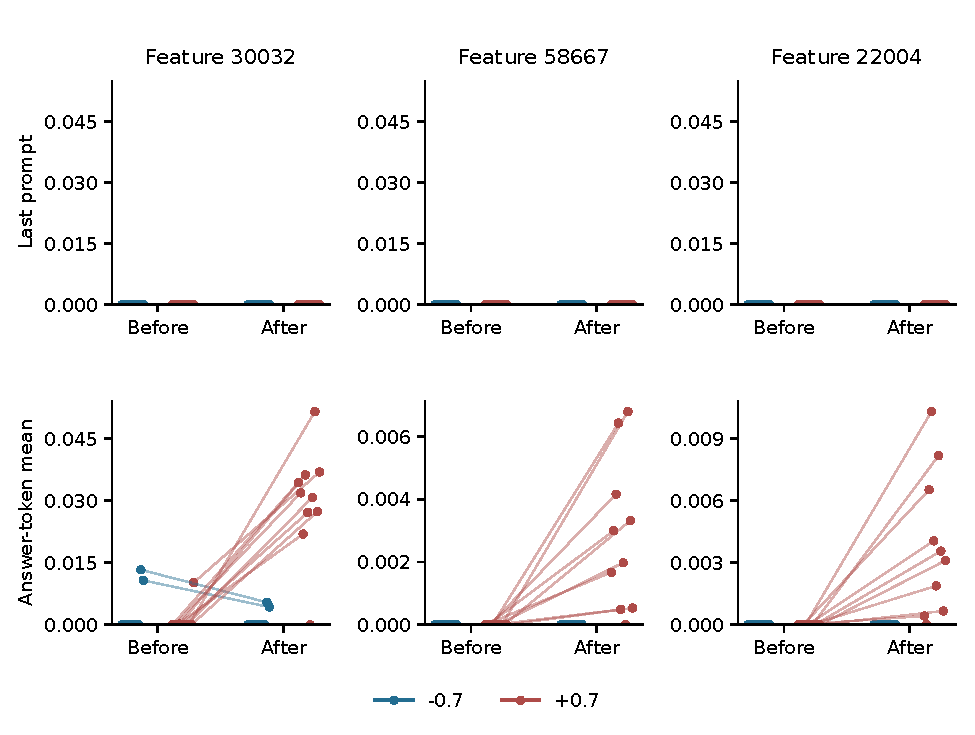
\includegraphics[width=\linewidth]{../evidence/figure_presentation/native_reencoding_1.pdf}
\caption{\textbf{How active each steered feature is, before and after the edit.}
The six features are shown in two groups of three (continued on the next
page). Each column is one feature, read back through the SAE during the
second turn; each line joins one seed's reading just before and just after
the edit (blue: $-0.7$; red: $+0.7$). Each panel contains ten seeds per sign.
Coincident zero readings overlap;
these lines are individual readings, not confidence intervals.
In each group, the top row shows the last prompt position,
just before the model starts its answer. All six features read zero there
before the edit, and only 23893 crosses its threshold under $+0.7$. Bottom
row: the average over the answer's tokens, excluding the final one. The
positive push raises every feature at some tokens, and the negative push
reduces the faint activity that was present, mostly to zero. A feature that
reads zero cannot fall further, so negative steering has little to remove.
Vertical scales differ across features. The quantities are SAE activations,
not probabilities of deception or subjective experience.}
\label{fig:native-reencoding}
\end{figure}

\begin{figure}[p]
\ContinuedFloat
\centering
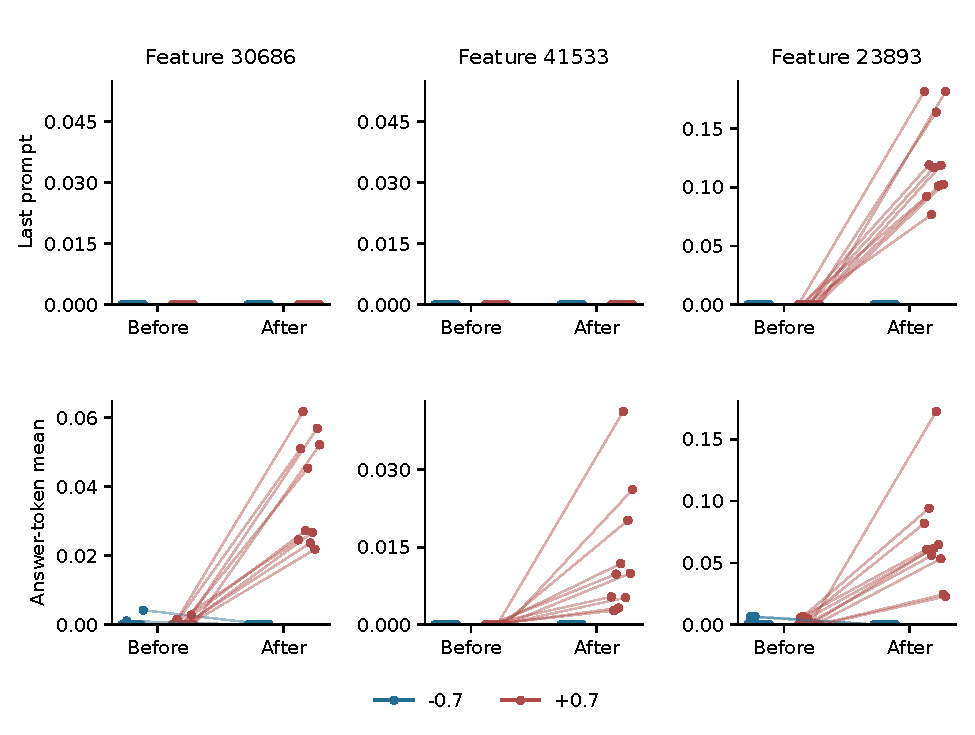
\includegraphics[width=\linewidth]{../evidence/figure_presentation/native_reencoding_2.pdf}
\caption[]{\textbf{How active each steered feature is, before and after the
edit (continued).} Remaining three features, with the same conventions:
blue $-0.7$, red $+0.7$; ten seeds per sign in each panel. Top: last prompt
position. Bottom: mean over answer tokens, excluding the final token.
Vertical scales differ across features; coincident zero readings overlap.}
\end{figure}

\subsection{Readout equations and all comparison mappings}
\label{app:jlens-details}

The Jacobian lens \citep{gurnee2026workspace} supplies a fixed, corpus-averaged linear transport from an
intermediate residual state toward the model's output representation. Applying
normalization and selected unembedding rows then gives token-indexed readout
scores. We use the released transport, not a new Jacobian fitted to these
outcomes. The scores are not calibrated probabilities of the named concepts.
For a transport $T_\ell$ and selected unembedding rows $W_V$, the gain-free
linear readout obeys
\[
 \ell^{\rm lin}_T(h_\ell+\delta h_\ell)
 -\ell^{\rm lin}_T(h_\ell)=W_V T_\ell\delta h_\ell.
\]
At the edited layer, agreement with the injected-vector prediction is thus
an implementation check. Further downstream, $\delta h_\ell$ reflects the
intervening computation, but projecting it does not by itself establish its
causal role in a later answer. The normalized scores reported below are
$W_V\operatorname{RMSNorm}(T_\ell h_\ell)$, a distinct readout.

Forty prospectively selected cases retain same-prefix clean and edited
executions at layers 50, 65 and 78. They cover both signs, the six individual
coordinates, the target aggregate and all matched panels, with two fixed
seeds. Each case is replayed on both its zero-intervention and steered source
history. Identity transport and five fixed random-J transports accompany the
pinned Jacobian lens. These are descriptive internal measurements, not
additional independent behavioral trials.
The capture inventory was frozen; the secondary reductions and displays
were added separately and are not confirmatory mechanism endpoints.

The displayed readout contrast is the target aggregate's paired normalized-logit
change minus the equal mean of the three matched-panel changes, averaged over
the two seeds at turn 2's final prompt position. On the common zero-source
history, the layer-78 deception-lexicon contrast is
$\SourceJZeroPositiveDeceptionJacobian{}$ for $+0.5$ steering with J-lens and
$\SourceJZeroPositiveDeceptionIdentity{}$ with identity; for $-0.5$ steering,
it is $\SourceJZeroNegativeDeceptionJacobian{}$ and
$\SourceJZeroNegativeDeceptionIdentity{}$, respectively. Identity therefore also detects the
downstream footprint: this is not evidence for unique diagnostic power of
J-lens. At the intervention site, the gain-free linear
readout difference is largely predicted by the known injected decoder vector.
That agreement checks the intervention and readout; it is not discovery of a
hidden belief. The normalized readout also includes learned RMSNorm gains
and a state-dependent denominator, so subtracting its values from linear
scores would not isolate a normalization effect.

Table~\ref{tab:source-jlens} reports every lexicon group, not just deception.
In this two-seed summary, positive steering raises the honesty readout as
well as the deception readout relative to the matched panels. These token
scores cannot be interpreted as a calibrated honesty-versus-deception axis.

\begin{table}[htbp]
\centering
\caption{\textbf{Downstream footprint with semantic and transport comparators.}
Both signs of the fixed-six aggregate, on the shared zero-source history.
The random-transport range is descriptive, not a confidence interval.}
\label{tab:source-jlens}
% Generated by evidence/build_source_jlens_table.py; do not edit numbers manually.
% Source release commit: ef10a0349e047272212319dadf484c3281e60bbe
% Source alignment manifest SHA256: e7d1f0565e44d655bc5c6986fff3a3f44c0b63ac4f8d115d572fc5ab666a3a0e
% J overview SHA256: d347a96eac176019b4b22e54592bc7e01a92133c842d284f284a82b04345e4a9
\begingroup
\small
\begin{tabular}{lrrrrr}
\hline
Lexicon group & Dose & J & Identity & Random-J min & Random-J max \\
\hline
Deception & $-0.5$ & $-0.4935$ & $-0.3367$ & $-0.0653$ & $+0.1184$ \\
Deception & $+0.5$ & $+0.5304$ & $+0.3568$ & $-0.1185$ & $+0.0576$ \\
Experience & $-0.5$ & $-0.1314$ & $-0.1006$ & $-0.1138$ & $+0.1751$ \\
Experience & $+0.5$ & $+0.1356$ & $+0.1248$ & $-0.1809$ & $+0.0867$ \\
Hedging & $-0.5$ & $-0.0544$ & $-0.0516$ & $-0.0212$ & $+0.0688$ \\
Hedging & $+0.5$ & $+0.0568$ & $+0.0547$ & $-0.0475$ & $+0.0170$ \\
Honesty & $-0.5$ & $-0.1802$ & $-0.1224$ & $-0.0277$ & $+0.0623$ \\
Honesty & $+0.5$ & $+0.2023$ & $+0.1380$ & $-0.0457$ & $+0.0109$ \\
Intervention & $-0.5$ & $-0.0418$ & $-0.0777$ & $-0.0766$ & $+0.0955$ \\
Intervention & $+0.5$ & $+0.0719$ & $+0.1139$ & $-0.1117$ & $+0.0670$ \\
Roleplay & $-0.5$ & $-0.2656$ & $-0.1979$ & $-0.0721$ & $+0.1028$ \\
Roleplay & $+0.5$ & $+0.2930$ & $+0.2352$ & $-0.0892$ & $+0.0702$ \\
Unrelated & $-0.5$ & $+0.0550$ & $+0.0124$ & $-0.0621$ & $+0.0212$ \\
Unrelated & $+0.5$ & $-0.0750$ & $-0.0188$ & $-0.0184$ & $+0.0383$ \\
\hline
\end{tabular}
\par\smallskip
\footnotesize
Zero history, layer 78, turn 2 last prompt. Values are target minus the equal mean of three control panels,
in normalized-logit units; each panel averages two seeds. Descriptive only, with no confidence intervals.
J denotes the Jacobian transport. Random-J min/max span all five fixed random transports;
this is a transport range, not uncertainty. Source-reduced case values, not raw-state-to-J reconstruction.
NA preserves missingness; a random range requires all five transports.
\par
\endgroup

\end{table}

All four sign-by-source-history heatmaps are released, including identity
and every random-J control. The clean-source-history comparisons share the
prefix across target and control panels; steered-source-history comparisons
do not, because each panel has already generated a different first turn.
No readout is treated as a mediator merely because it changes. In this
experiment the internal footprint is visible without a corresponding large
observed report-label contrast under the alternative wording. A causal account of report production would require
a held-out intervention on the candidate downstream computation, together
with matched ablation and restoration controls.

The \nativeartifact{data/berg_source_replication/source_aligned_v1_20261001/RELEASE_MANIFEST.json}{release manifest}
binds all raw outputs and source-rendered figures. The companion checker
reconstructs label counts and paired point estimates from raw-bound indices,
and the displayed J-lens contrasts from source-reduced case values. It does
not independently recompute bootstrap intervals, re-encode activations,
reconstruct state-to-J readouts or redraw source figures.
